%! TEX program = pdflatex

\documentclass[oneside,solution]{karazin-control-assign}

\usepackage[utf8]{inputenc}
\usepackage[english,ukrainian]{babel}

\title{Домашня Робота}
\author{Захаров Дмитро}
\studentID{МП-31}
\instructor{Сморцова Т.І.}
\date{\today}
\duedate{23:59 30 квітня, 2024}
\assignno{2}
\semester{Весняний семестр 2024}
\mainproblem{Варіант 3}

\begin{document}

\maketitle

% \startsolution[print]

\problem{Канонічний вид системи}

\hspace{20px}\textit{Умова.} Чи є система
\begin{equation}
    \begin{cases}
        \dot{x}_1 = x_2 + 2x_3 - u \\
        \dot{x}_2 = 2x_1 + x_2 - x_3 + 2x_4 \\
        \dot{x}_3 = 3x_3 - 3x_4 - 3u \\
        \dot{x}_4 = x_3 - x_4
    \end{cases}
\end{equation}
повністю керованою? Привести систему до канонічного вигляду. Чи є ця система стабілізованою?

\textit{Розв'язання.} Нехай $\mathbf{x}=(x_1,x_2,x_3,x_4)$, тоді система має стандартний вигляд
\begin{equation}
    \dot{\mathbf{x}} = \boldsymbol{A}\mathbf{x} + \boldsymbol{\beta}u, \; \boldsymbol{A} = \begin{bmatrix}
        0 & 1 & 2 & 0 \\
        2 & 1 & -1 & 2 \\
        0 & 0 & 3 & -3 \\
        0 & 0 & 1 & -1 
    \end{bmatrix}, \; \boldsymbol{\beta} = \begin{bmatrix}
        -1 \\ 0 \\ -3 \\ 0
    \end{bmatrix}
\end{equation}

Для аналізу повної керованості складаємо матрицю Калмана:
\begin{equation}
    \boldsymbol{K} = [\boldsymbol{\beta} \parallel \boldsymbol{A\beta} \parallel \boldsymbol{A}^2\boldsymbol{\beta} \parallel \boldsymbol{A}^3\boldsymbol{\beta}]
\end{equation}

Далі знаходимо степені матриці:
\begin{equation}
    \boldsymbol{A}^2 = \begin{bmatrix}
        2 & 1 & 5 & -4 \\
        2 & 3 & 2 & 3 \\
        0 & 0 & 6 & -6 \\
        0 & 0 & 2 & -2
    \end{bmatrix}, \; \boldsymbol{A}^3 = \begin{bmatrix}
        2 & 3 & 14 & -9 \\
        6 & 5 & 10 & -3 \\
        0 & 0 & 12 & -12 \\
        0 & 0 & 4 & -4
    \end{bmatrix}
\end{equation}

Отже, матриця Калмана має вигляд:
\begin{equation}
    \boldsymbol{K} = \begin{bmatrix}
        -1 & -6 & -17 & -44\\
        0  & 1 & -8 & -36\\
        -3 & -9 & -18 & -36\\
        0 & -3 & -6 & -12
    \end{bmatrix}
\end{equation}

Покажемо, що система не є повністю керованою, тобто $\text{rang}(\boldsymbol{K}) < n=4$. Для цього починаємо перетворювати матрицю:
\begin{gather}
    \boldsymbol{K} = \begin{bmatrix}
        -1 & -6 & -17 & -44 \\
        0  & 1 & -8 & -36 \\
        -3 & -9 & -18 & -36 \\
        0 & -3 & -6 & -12
    \end{bmatrix} \xrightarrow[R_3/(-3)]{R_4/(-3)} \begin{bmatrix}
        -1 & -6 & -17 & -44 \\
        0  & 1 & -8 & -36 \\
        1 & 3 & 6 & 12 \\
        0 & 1 & 2 & 4
    \end{bmatrix} \nonumber \\
    \xrightarrow[R_3-R_1]{R_1 \times (-1)} \begin{bmatrix}
        1 & 6 & 17 & 44 \\
        0  & 1 & -8 & -36 \\
        0 & -3 & -11 & -32 \\
        0 & 1 & 2 & 4
    \end{bmatrix} \xrightarrow[R_3+3R_2]{R_4-R_2} \begin{bmatrix}
        1 & 6 & 17 & 44 \\
        0  & 1 & -8 & -36 \\
        0 & 0 & -35 & -140 \\
        0 & 0 & 10 & 40
    \end{bmatrix} \nonumber \\
    \xrightarrow[]{3.5R_4+R_2} \begin{bmatrix}
        1 & 6 & 17 & 44 \\
        0  & 1 & -8 & -36 \\
        0 & 0 & -35 & -140 \\
        0 & 0 & 0 & 0
    \end{bmatrix} \implies \det \boldsymbol{K} = 0
\end{gather}

Отже, система не є повністю керованою, бо $\text{rang}(\boldsymbol{K}) = 3 < 4$. Тому, введемо два лінійних підпростори:
\begin{equation}
    \mathcal{L} = \text{span}\left\{ \begin{bmatrix}
        -1 \\ 0 \\ -3 \\ 0
    \end{bmatrix},\begin{bmatrix}
        -6 \\ 1 \\ -9 \\ -3
    \end{bmatrix},\begin{bmatrix}
        -17 \\ -8 \\ -18 \\ -6
    \end{bmatrix}\right\}, \; \dim \mathcal{L} = 3
\end{equation}

та ортогональний підпростір $\mathcal{L}^{\perp}$. Оскільки $\dim \mathcal{L}^{\perp} = 1$, то $\mathcal{L}^{\perp} = \text{span} \{\boldsymbol{\alpha}\}$, тому знайдемо $\boldsymbol{\alpha}$ з умови $\boldsymbol{\alpha} \perp \boldsymbol{\beta},\boldsymbol{A\beta},\boldsymbol{A}^2\boldsymbol{\beta}$. Для цього запишемо систему:
\begin{equation}
    \langle \boldsymbol{\alpha}, \boldsymbol{A}^n\boldsymbol{\beta} \rangle = 0, \; n \in \{0,1,2\}
\end{equation}

Або, аналогічно:
\begin{equation}
    \begin{cases}
        -\alpha_1 - 3\alpha_3 = 0 \\
        -6\alpha_1 + \alpha_2 - 9\alpha_3 - 3\alpha_4 = 0 \\
        -17\alpha_1 - 8\alpha_2 - 18\alpha_3 - 6\alpha_4=0
    \end{cases}
\end{equation}

З першого рівняння $\alpha_1=-3\alpha_3$, підставляючи у два наступних:
\begin{equation}
    \begin{cases}
        \alpha_2 + 9\alpha_3 - 3\alpha_4 = 0 \\
        33\alpha_3 - 8\alpha_2 - 6\alpha_4 = 0
    \end{cases}
\end{equation}

З другого $\alpha_2=3\alpha_4-9\alpha_3$, тому $33\alpha_3-24\alpha_4+72\alpha_3-6\alpha_4=0$ або просто $105\alpha_3-30\alpha_4=0 \implies \alpha_4 = \frac{7}{2}\alpha_3$. Тому остаточно (якщо покласти $x_3=t$):
\begin{equation}
    \boldsymbol{\alpha} = \begin{bmatrix}
        -3 \\ 3/2 \\ 1 \\ 7/2
    \end{bmatrix}t = \begin{bmatrix}
        -6 \\ 3 \\ 2 \\ 7
    \end{bmatrix}\frac{t}{2}
\end{equation}

Отже покладемо $t=2$ і в такому разі $\boldsymbol{\alpha} = (-6,3,2,7)$. 

Далі вектор $\mathbf{c}$ знайдемо з умови $\mathbf{c} \perp \boldsymbol{\beta},\mathbf{c} \perp \boldsymbol{A}\boldsymbol{\beta},\mathbf{c} \not\perp \boldsymbol{A}^2\boldsymbol{\beta}$. Для цього, наприклад, задамо систему
\begin{equation}
    \langle \mathbf{c}, \boldsymbol{\beta} \rangle = \langle \mathbf{c}, \boldsymbol{A}\boldsymbol{\beta} \rangle = 0, \; \langle \mathbf{c}, \boldsymbol{A}^2\boldsymbol{\beta} \rangle = 10 \neq 0
\end{equation}

Далі розв'язання системи майже ідентичне, тому наведу проміжний результат при $x_3=t$:
\begin{equation}
    \mathbf{c} = \begin{bmatrix}
        -3t \\ \frac{1}{2}(-2+3t) \\ t \\ \frac{1}{6}(-2+21t)
    \end{bmatrix}
\end{equation}

При $t=0$ маємо $\mathbf{c} = (0,-1,0,-1/3)$. Тому в якості вектора візьмемо $(0,3,0,1)$\footnote{Тільки в цьому випадку скалярний добуток $\langle \mathbf{c},\boldsymbol{A}^2\boldsymbol{\beta}\rangle$ зміниться, але не стане нулевим.}.

Нарешті, матриця перетворення:
\begin{equation}
    \boldsymbol{F} = \begin{bmatrix}
        \boldsymbol{\alpha}^{\top} \\
        \mathbf{c}^{\top} \\
        \mathbf{c}^{\top}\boldsymbol{A} \\
        \mathbf{c}^{\top}\boldsymbol{A}^2
    \end{bmatrix} = \begin{bmatrix}
        -6 & 3 & 2 & 7 \\
        0 & 3 & 0 & 1 \\
        6 & 3 & -2 & 5 \\
        6 & 9 & 8 & 7
    \end{bmatrix}
\end{equation}

Тому, якщо перейдемо до $\mathbf{z}=\boldsymbol{F}\mathbf{x}$, то маємо систему
\begin{equation}
    \dot{\mathbf{z}} = \hat{\boldsymbol{A}}\mathbf{z} + \hat{\boldsymbol{\beta}}u, \; \hat{\boldsymbol{A}} = \boldsymbol{FAF}^{-1}, \; \hat{\boldsymbol{\beta}} = \boldsymbol{F}\mathbf{b}
\end{equation}

Обернена матриця:
\begin{equation}
    \boldsymbol{F}^{-1} = \begin{bmatrix}
        -1/15 & -1/10 & 1/15 & 1/30 \\
        -1/30 & 2/5 & -1/30 & 0 \\
        0 & -1/5 & -1/10 & 1/10 \\
        1/10 & -1/5 & 1/10 & 0
    \end{bmatrix}
\end{equation}

Тому, після множення, матриці ``з шапками'':
\begin{equation}
    \hat{\boldsymbol{A}} = \begin{bmatrix}
        -1 & 0 & 0 & 0\\
        0 & 0 & 1 & 0 \\
        0 & 0 & 0 & 1 \\
        -3 & 0 & -4 & 4
    \end{bmatrix}, \hat{\boldsymbol{\beta}} = \begin{bmatrix}
        0 \\ 0 \\ 0 \\ -30
    \end{bmatrix}
\end{equation}

Отже, наша система в канонічному вигляді:
\begin{equation}
    \begin{cases}
        \dot{z}_1 = -z_1 \\
        \dot{z}_2 = z_3 \\
        \dot{z}_3 = z_4 \\
        \dot{z}_4 = -3z_1 - 4z_3 + 4z_4 -30u
    \end{cases}
\end{equation}

Дійсно отримали некеровану частину $\dot{z}_1=-z_1$ і керовану трьома рівняннями нижче. Тепер щоб перевірити, чи є система стабілізованою, потрібно перевірити наступну умову:
\begin{equation}
    \forall \lambda \in \sigma(\boldsymbol{A}), \text{Re}(\lambda) \geq 0: \mathcal{K}(\lambda) \subset \mathcal{L} = \text{span}\{\boldsymbol{\beta},\boldsymbol{A\beta},\boldsymbol{A}^2\boldsymbol{\beta}\}
\end{equation}

Отже, знаходимо спектр матриці $\boldsymbol{A}$. Характеристичний поліном:
\begin{equation}
    \chi_A(\lambda) = \det\begin{bmatrix}
        -\lambda & 1 & 2 & 0 \\
        2 & 1-\lambda & -1 & 2 \\
        0 & 0 & 3-\lambda & -3 \\
        0 & 0 & 1 & -1-\lambda
    \end{bmatrix} = (\lambda-2)^2\lambda(1+\lambda)
\end{equation}

Отже маємо три власних числа: $\lambda_1=2$ кратності 2, та $\lambda_2=0,\lambda_3=-1$ кратності $1$. Оскільки $\lambda_3<0$, то перевірити потрібно лише $\lambda_1,\lambda_2$. Почнемо з $\lambda_2$. Відповідним кореневим підпростором є ядро $\text{ker}(\boldsymbol{A})$, тому запишемо:
\begin{equation}
    \begin{cases}
        x_2 + 2x_3 = 0 \\
        2x_1 + x_2 - x_3 + 2x_4 = 0 \\
        3x_3 - 3x_4 = 0\\
        x_3 - x_4 = 0
    \end{cases}
\end{equation}

З останніх двох рівнянь $x_3=x_4$. Тоді з першого $x_2=-2x_3$, а тому для третього $2x_1 = -x_2+x_3-2x_4=2x_3+x_3-2x_3=x_3$. Таким чином,
\begin{equation}
    \mathcal{K}(0) = \text{ker}(\boldsymbol{A}) = \{(1,-4,2,2)\mu: \mu \in \mathbb{R}\}
\end{equation}

Чи є це підпростором $\mathcal{L}$? Так, оскільки
\begin{equation}
    \begin{bmatrix}
        1 \\ -4 \\ 2 \\ 2
    \end{bmatrix} = \frac{4}{3}\begin{bmatrix}
        -1 \\ 0 \\ -3 \\ 0
    \end{bmatrix} - \frac{4}{3}\begin{bmatrix}
        -6 \\ 1 \\ -9 \\ -3
    \end{bmatrix} + \frac{1}{3}\begin{bmatrix}
        -17 \\ -8 \\ -18 \\ -6
    \end{bmatrix}
\end{equation}

Тепер перевіримо $\lambda_1=2$. Відповідний кореневий підпростір:
\begin{equation}
    \mathcal{K}(2) = \text{ker}((\boldsymbol{A}-2\boldsymbol{E})^2)
\end{equation}

Порахувавши, маємо:
\begin{equation}
    (\boldsymbol{A}-2\boldsymbol{E})^2 = \begin{bmatrix}
        6 & -3 & -3 & -4 \\
        -6 & 3 & 6 & -5\\
        0 & 0 & -2 & 6 \\
        0 & 0 & -2 & 6
    \end{bmatrix}
\end{equation}

Тому для знаходження ядра знаходимо:
\begin{equation}
    \begin{cases}6x_1 - 3x_2 - 3x_3 - 4x_4 = 0\\
    -6x_1 + 3x_2 + 6x_3 - 5x_4 = 0\\
    -x_3 + 3x_4 = 0
    \end{cases}
\end{equation}

З останнього рівняння $x_3=3x_4$. Тому перші два рівняння перетворюються у $\begin{cases}
    6x_1 - 3x_2 = 13x_4 \\ 
    -6x_1+3x_2 = -13x_4
\end{cases}$. Отже бачимо, що 
\begin{equation}
    \mathcal{K}(2) = \{((13\mu+3\nu)/6,\nu,3\mu,\mu): \mu,\nu \in \mathbb{R}\} = \{(13\mu+3\nu,6\nu,18\mu,6\mu): \mu,\nu \in \mathbb{R}\}
\end{equation}

Таким чином, 
\begin{equation}
    \mathcal{K}(2) = \text{span}\left\{ \begin{bmatrix}
        13 \\ 0 \\ 18 \\ 6
    \end{bmatrix}, \begin{bmatrix}
        1 \\ 2 \\ 0 \\ 0
    \end{bmatrix}\right\}
\end{equation}

Чи $\mathcal{K}(2) \subset \mathcal{L}$? Так, оскільки
\begin{gather}
    \begin{bmatrix}
        1 \\ 2 \\ 0 \\ 0
    \end{bmatrix} = 0\begin{bmatrix}
        -1 \\ 0 \\ -3 \\ 0
    \end{bmatrix} + \frac{2}{5}\begin{bmatrix}
        -6 \\ 1 \\ -9 \\ -3
    \end{bmatrix} - \frac{1}{5}\begin{bmatrix}
        -17 \\ -8 \\ -18 \\ -6
    \end{bmatrix} \\
    \begin{bmatrix}
        13 \\ 0 \\ 18 \\ 6
    \end{bmatrix} = 0\begin{bmatrix}
        -1 \\ 0 \\ -3 \\ 0
    \end{bmatrix} - \frac{8}{5}\begin{bmatrix}
        -6 \\ 1 \\ -9 \\ -3
    \end{bmatrix} - \frac{1}{5}\begin{bmatrix}
        -17 \\ -8 \\ -18 \\ -6
    \end{bmatrix}
\end{gather}

Отже, система дійсно є стабілізованою.

\problem{Стабілізація системи}

\hspace{20px}\textit{Умова.} Стабілізувати систему
\begin{equation}
    \begin{cases}
        \dot{x}_1 = 2x_1 - x_2 + 2x_3 \\
        \dot{x}_2 = x_1 + 2x_3 + u \\
        \dot{x}_3 = -2x_1 + x_2 - x_3
    \end{cases}
\end{equation}

\textit{Розв'язання.} Будемо обирати керування у вигляді $u=p_1x_1+p_2x_2+p_3x_3$, щоб власні значення системи знаходились у лівій півплощині. Маємо:
\begin{equation}
    \dot{\mathbf{x}} = \boldsymbol{A}(p_1,p_2,p_3)\mathbf{x}, \; \boldsymbol{A}(p_1,p_2,p_3) = \begin{bmatrix}
        2 & -1 & 2 \\
        p_1+1 & p_2 & p_3+2 \\
        -2 & 1 & -1
    \end{bmatrix}
\end{equation}

Нам потрібно, щоб $\forall \lambda \in \sigma(\boldsymbol{A}): \text{Re}(\lambda) < 0$. Для цього випишемо характеристичний поліном:
\begin{gather}
    \chi_A(\lambda \mid p_1,p_2,p_3) = \det \begin{bmatrix}
        2 - \lambda & -1 & 2 \\
        p_1 + 1 & p_2 - \lambda & p_3 + 2 \\
        -2 & 1 & -1-\lambda
    \end{bmatrix} \nonumber \\
    =-\lambda^3 + (1+p_2)\lambda^2 - (1+p_1+p_2-p_3)\lambda + (1+p_1+2p_2)
\end{gather}

Нам потрібно підібрати набір $(p_1,p_2,p_3)$ так, щоб усі корені $\lambda$ мали від'ємну дійсну частину. Для цього, наприклад, підберемо коефіцієнти таким чином, щоб $\chi_A(\lambda \mid p_1,p_2,p_3) \equiv -(\lambda+1)^3$. Для цього має виконуватись:
\begin{equation}
    \begin{cases}
        1+p_2 = -3 \\
        1+p_1+p_2-p_3 = 3 \\
        1 + p_1 + 2p_2 = -1
    \end{cases}
\end{equation}

З першого рівняння $p_2=-4$, тоді з третього $p_1=-2-2p_2=6$, а з другого нарешті $p_3=-2+p_1+p_2=0$. В такому разі, наше керування має вигляд:
\begin{equation}
    u = 6x_1 - 4x_2
\end{equation}

\problem{Кускове-стале керування}

\hspace{20px}\textit{Умова.} Знайти кусково стале керування з точкою перемикання $t=1$, яке за проміжок часу $[0,3]$ переводить точку $(0,0)$ в точку $(-2,5)$ в силу системи $\begin{cases}
    \dot{x}_1 = 2u \\ \dot{x}_2 = 4x_1-u
\end{cases}$. Виписати траєкторію системи, за якою відбувається цей перехід.

\textit{Розв'язання.} Як сказано в умові, обираємо кускове-стале керування:
\begin{equation}
    u(t) = \begin{cases}
        \alpha, & t \in [0,1), \\
        \beta, & t \in [1,3]
    \end{cases}
\end{equation}

Розв'яжемо диференціальне рівняння, підставивши $u \equiv u_0$. З першого рівняння $x_1(t) = 2u_0 t + c_1$. Підставляючи у друге, маємо:
\begin{equation}
    \dot{x}_2 = 8u_0t + 4c_1 - u_0 \implies x_2(t) = 4u_0t^2 + (4c_1 - u_0)t + c_2
\end{equation}

Отже, траєкторія має вигляд:
\begin{gather}
    \begin{cases}
        x_1(t) = 2\alpha t + c_1 \\
        x_2(t) = 4\alpha t^2 + (4c_1 - \alpha)t + c_2
    \end{cases}, \; t \in [0,1) \\
    \begin{cases}
        x_1(t) = 2\beta t + \widetilde{c}_1 \\
        x_2(t) = 4\beta t^2 + (4\widetilde{c}_1 - \beta)t + \widetilde{c}_2
    \end{cases}, \; t \in [1,3]
\end{gather}

Отже, залишилось лише знайти коефіцієнти $(\alpha,\beta,c_1,c_2,\widetilde{c}_1,\widetilde{c}_2)$, для цього потрібно $6$ рівнянь. Чотири рівняння отримаємо з умов $\mathbf{x}(0)=(0,0)$ та $\mathbf{x}(3)=(-2,5)$. Ще дві умови задамо з умови неперервності траєкторії:
\begin{equation}
    \lim_{t \to 1^-}\mathbf{x}(t) = \lim_{t \to 1^+}\mathbf{x}(t)
\end{equation}

Отже, складаємо умови у стопку:
\begin{equation}
    \mathbf{x}(0) = (0,0):  \begin{cases}
        c_1 = 0 \\ c_2 = 0
    \end{cases}
\end{equation}
\begin{equation}
    \mathbf{x}(3) = (-2,5): \begin{cases}
        6\beta + \widetilde{c}_1 = -2 \\
        36\beta + 3(4\widetilde{c}_1-\beta) + \widetilde{c}_2 = 5
    \end{cases}
\end{equation}
\begin{equation}
    \lim_{t \to 1^-}\mathbf{x}(t) = \lim_{t \to 1^+}\mathbf{x}(t): \begin{cases}
        2\alpha + c_1 = 2\beta + \widetilde{c}_1 \\ 
        4\alpha + 4c_1 - \alpha + c_2 = 4\beta + 4\widetilde{c}_1-\beta + \widetilde{c}_2 
    \end{cases}
\end{equation}

Отже, $c_1=c_2=0$ знаходимо одразу, а для інших значень маємо систему:
\begin{equation}
    \begin{cases}
        2\alpha = 2\beta + \widetilde{c}_1 \\
        3\alpha = 3\beta + 4\widetilde{c}_1 + \widetilde{c}_2 \\
        6\beta + \widetilde{c}_1 = -2 \\
        33\beta + 12\widetilde{c}_1 + \widetilde{c}_2 = 5
    \end{cases}
\end{equation}

Далі розв'язуємо. З першого рівняння $\widetilde{c}_1 = 2\alpha-2\beta$, підставляємо у всі інші:
\begin{equation}
    \begin{cases}
        3\alpha = 3\beta + 8\alpha - 8\beta + \widetilde{c}_2 \\
        6\beta + 2\alpha-2\beta = -2 \\
        33\beta + 24\alpha - 24\beta + \widetilde{c}_2 = 5
    \end{cases}
\end{equation}

Або, якщо спростити:
\begin{equation}
    \begin{cases}
        5\beta = 5\alpha + \widetilde{c}_2 \\
        2\beta + \alpha = -1 \\
        9\beta + 24\alpha + \widetilde{c}_2 = 5
    \end{cases}
\end{equation}

З другого рівняння $\alpha=-1-2\beta$, тому
\begin{equation}
    \begin{cases}
        5\beta = -5-10\beta + \widetilde{c}_2 \\
        9\beta - 24 - 48\beta + \widetilde{c}_2 = 5
    \end{cases} \implies \begin{cases}
        15\beta - \widetilde{c}_2 = -5 \\
        -39\beta + \widetilde{c}_2 = 29
    \end{cases}
\end{equation}

Звідси отримуємо розв'язок $(\beta,\widetilde{c}_2)=(-1,-10)$. Звідси $\alpha=1$ і $\widetilde{c}_1 = 4$. Отже, остаточно наша траєкторія:
\begin{equation}
    \begin{cases}
        x_1(t) = 2t \\
        x_2(t) = 4t^2 - t 
    \end{cases}, \; t \in [0,1)
\end{equation}
\begin{equation}
    \begin{cases}
        x_1(t) = -2t + 4 \\
        x_2(t) = -4t^2 + 17t - 10
    \end{cases}, \; t \in [1,3]
\end{equation}

з керуванням $u(t) = \begin{cases}
    1, & t \in [0,1) \\
    -1, & t \in [1,3]
\end{cases}$. Траєкторію можна побачити на Рисунку \ref{fig:problem-3}. Як видно траєкторія дійсно неперервна, починається в $(0,0)$ і входить в точку $(-2,5)$, а ``перелом'' відбувається в точці $(2,3)$, що дійсно відповідає моменту часу $t=1$ у рівняннях зверху.

\begin{figure}
    \centering
    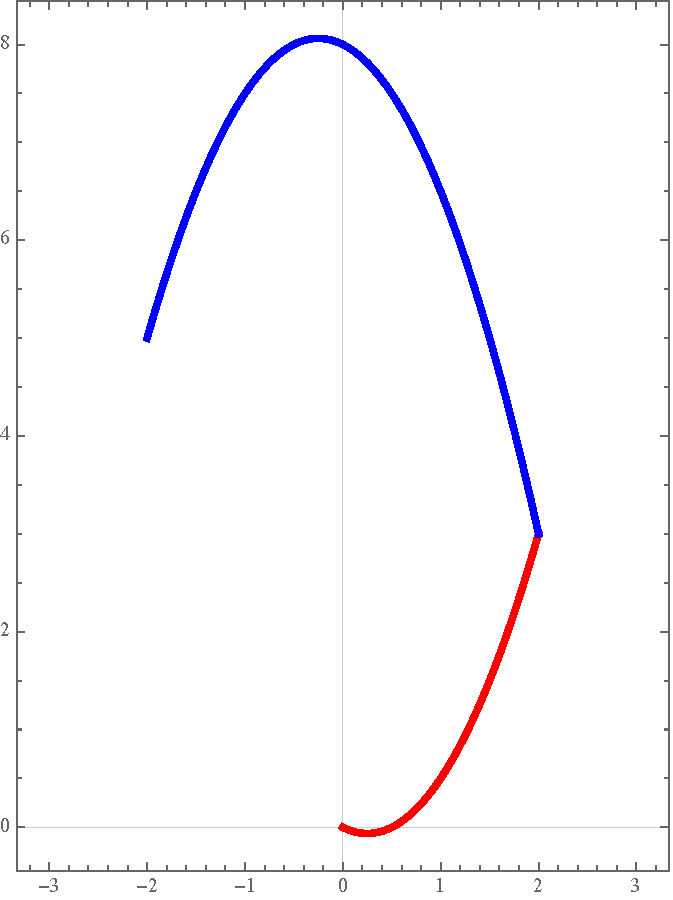
\includegraphics[width=0.4\textwidth]{figure.pdf}
    \caption{Графік траєкторії з задачі 3 при керуванні $u(t)=1$ якщо $t \in [0,1)$ та $u(t)=-1$ при $t \in [1,3]$.}
    \label{fig:problem-3}
\end{figure}

\end{document}
